% !Mode:: "TeX:UTF-8"
\documentclass{mcmthesis}
% Configurations
% !Mode:: "TeX:UTF-8"

% ------- Packages -------
\usepackage{palatino}    % Palatino/Helvetica/TXTT and Greek replacements
\usepackage{lipsum}        % 生成测试文本
\usepackage{hologo}        % TeX符号
\usepackage{amsthm}        % Theorem
    \newtheorem{thm}{Theorem}[section]
    \newtheorem{cor}{Corollary}[section]
    \newtheorem{defn}{Definition}[section]
\usepackage{fontawesome}   % 图标
\usepackage{hyperref}      % 超链接
% \usepackage{PyLaTeX}       % https://github.com/Iydon/LaTeX_template/tree/master/PyLaTeX
%     \pylatexpycmd{python3} % Python cmd name
%     \pylatexdoit

% ------- Symbols -------
% !Mode:: "TeX:UTF-8"
\usepackage{xspace}
\usepackage{mathrsfs}

% Fette Kleinbuchstaben (fuer Vektoren)
\newcommand{\Va}{{\mathbf{a}}}
\newcommand{\Vb}{{\mathbf{b}}}
\newcommand{\Vc}{{\mathbf{c}}}
\newcommand{\Vd}{{\mathbf{d}}}
\newcommand{\Ve}{{\mathbf{e}}}
\newcommand{\Vf}{{\mathbf{f}}}
\newcommand{\Vg}{{\mathbf{g}}}
\newcommand{\Vh}{{\mathbf{h}}}
\newcommand{\Vi}{{\mathbf{i}}}
\newcommand{\Vj}{{\mathbf{j}}}
\newcommand{\Vk}{{\mathbf{k}}}
\newcommand{\Vl}{{\mathbf{l}}}
\newcommand{\Vm}{{\mathbf{m}}}
\newcommand{\Vn}{{\mathbf{n}}}
\newcommand{\Vo}{{\mathbf{o}}}
\newcommand{\Vp}{{\mathbf{p}}}
\newcommand{\Vq}{{\mathbf{q}}}
\newcommand{\Vr}{{\mathbf{r}}}
\newcommand{\Vs}{{\mathbf{s}}}
\newcommand{\Vt}{{\mathbf{t}}}
\newcommand{\Vu}{{\mathbf{u}}}
\newcommand{\Vv}{{\mathbf{v}}}
\newcommand{\Vw}{{\mathbf{w}}}
\newcommand{\Vx}{{\mathbf{x}}}
\newcommand{\Vy}{{\mathbf{y}}}
\newcommand{\Vz}{{\mathbf{z}}}

% Small bold math characters
\newcommand{\Ba}{{\boldsymbol{a}}}
\newcommand{\Bb}{{\boldsymbol{b}}}
\newcommand{\Bc}{{\boldsymbol{c}}}
\newcommand{\Bd}{{\boldsymbol{d}}}
\newcommand{\Be}{{\boldsymbol{e}}}
\newcommand{\Bf}{{\boldsymbol{f}}}
\newcommand{\Bg}{{\boldsymbol{g}}}
\newcommand{\Bh}{{\boldsymbol{h}}}
\newcommand{\Bi}{{\boldsymbol{i}}}
\newcommand{\Bj}{{\boldsymbol{j}}}
\newcommand{\Bk}{{\boldsymbol{k}}}
\newcommand{\Bl}{{\boldsymbol{l}}}
\newcommand{\Bm}{{\boldsymbol{m}}}
\newcommand{\Bn}{{\boldsymbol{n}}}
\newcommand{\Bo}{{\boldsymbol{o}}}
\newcommand{\Bp}{{\boldsymbol{p}}}
\newcommand{\Bq}{{\boldsymbol{q}}}
\newcommand{\Br}{{\boldsymbol{r}}}
\newcommand{\Bs}{{\boldsymbol{s}}}
\newcommand{\Bt}{{\boldsymbol{t}}}
\newcommand{\Bu}{{\boldsymbol{u}}}
\newcommand{\Bv}{{\boldsymbol{v}}}
\newcommand{\Bw}{{\boldsymbol{w}}}
\newcommand{\Bx}{{\boldsymbol{x}}}
\newcommand{\By}{{\boldsymbol{y}}}
\newcommand{\Bz}{{\boldsymbol{z}}}

% Small bold characters with hat on top
\newcommand{\VaH}{\widehat{\mathbf{a}}}
\newcommand{\VbH}{\widehat{\mathbf{b}}}
\newcommand{\VcH}{\widehat{\mathbf{c}}}
\newcommand{\VdH}{\widehat{\mathbf{d}}}
\newcommand{\VeH}{\widehat{\mathbf{e}}}
\newcommand{\VfH}{\widehat{\mathbf{f}}}
\newcommand{\VgH}{\widehat{\mathbf{g}}}
\newcommand{\VhH}{\widehat{\mathbf{h}}}
\newcommand{\ViH}{\widehat{\boldsymbol \imath}}
\newcommand{\VjH}{\widehat{\boldsymbol \jmath}}
\newcommand{\VkH}{\widehat{\mathbf{k}}}
\newcommand{\VlH}{\widehat{\mathbf{l}}}
\newcommand{\VmH}{\widehat{\mathbf{m}}}
\newcommand{\VnH}{\widehat{\mathbf{n}}}
\newcommand{\VoH}{\widehat{\mathbf{o}}}
\newcommand{\VpH}{\widehat{\mathbf{p}}}
\newcommand{\VqH}{\widehat{\mathbf{q}}}
\newcommand{\VrH}{\widehat{\mathbf{r}}}
\newcommand{\VsH}{\widehat{\mathbf{s}}}
\newcommand{\VtH}{\widehat{\mathbf{t}}}
\newcommand{\VuH}{\widehat{\mathbf{u}}}
\newcommand{\VvH}{\widehat{\mathbf{v}}}
\newcommand{\VwH}{\widehat{\mathbf{w}}}
\newcommand{\VxH}{\widehat{\mathbf{x}}}
\newcommand{\VyH}{\widehat{\mathbf{y}}}
\newcommand{\VzH}{\widehat{\mathbf{z}}}


% ------- Command and Definition -------
% 正文摘要和控制页摘要名字修改
\def\abstractname{Abstract}
\def\sheetsummaryname{Summary}

% ------- Information -------
\mcmsetup{CTeX = false,         % 使用 CTeX 套装时,设置为 true
        tcn = 0710,             % 队伍控制号码
        problem = A,            % 选题
        sheet = true,           % 摘要页
        titleinsheet = true,    % 摘要页中的标题
        keywordsinsheet = true, % 摘要页中的关键字
        titlepage = true,       % 标题页
        abstract = true,        % 标题页中的摘要
        XeTeX = true,           % XeTeX编译
}
\title{The \LaTeX{} Template for MCM Version \MCMversion}
\author{Iydon, Svégio, Xylocis}
\date{\today}   % 导言区
% !Mode:: "TeX:UTF-8"
% ------- Warning -------
% LaTeX Font Warning: Some font shapes were not available, defaults substituted.
% TODO

% Package Fancyhdr Warning: \headheight is too small (12.0pt):
\setlength{\headheight}{27pt}    % Warning补丁
\begin{document}

% !Mode:: "TeX:UTF-8"
% 控制页摘要内容
% \begin{sheetsummary}
% \lipsum[1]
% \end{sheetsummary}

% 正文摘要内容
\begin{abstract}
\lipsum[2]
\end{abstract}

% 关键词
\begin{keywords}
\hologo{XeLaTeX}; 
\includegraphics{SUSTeX}; \jobname
\end{keywords} 
\maketitle
% Generate the Table of Contents, if it's needed.
\tableofcontents\newpage

% Examples.
% !Mode:: "TeX:UTF-8"

\section{Lists}
    % !Mode:: "TeX:UTF-8"
\subsection{Itemize}
\begin{itemize}
    \item Point A
    \item Point B
    \begin{itemize}
        \item part 1
        \item part 2
    \end{itemize}
    \item Point C
    \item Point D
\end{itemize}

\subsection{Enumerate}
\begin{enumerate}
    \item Point A
    \item Point B
    \begin{enumerate}
        \item part 1
        \item part 2
    \end{enumerate}
    \item Point C
    \item Point D
\end{enumerate}

\subsection{Enumerate (Roman Numerals)}
\begin{enumerate} [(I)]
	\item Point A
	\item Point B
	\begin{enumerate} [(i)]
        \item part 1
        \item part 2
	\end{enumerate}
	\item Point C
	\item Point D
\end{enumerate}

\section{Minipage}
    % !Mode:: "TeX:UTF-8"
\subsection{Minipage}
\begin{minipage}{0.1\linewidth}
    \flushright\color{blue}
	1 \\2 \\3 \\4 \\5 \\6 \\7 \\8 \\9 \\10 \\11 \\12 \\13 
\end{minipage}
\begin{minipage}{0.8\linewidth}
	\lipsum[1]
\end{minipage}

\section{Figures}
    % !Mode:: "TeX:UTF-8"
\subsection{Figures}
\begin{figure}[htb]
    \centering
    \begin{tabular}{cc}
        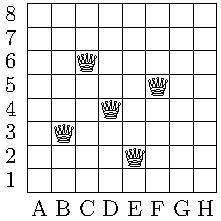
\includegraphics[scale=1]{examples/Chess1.pdf} &
        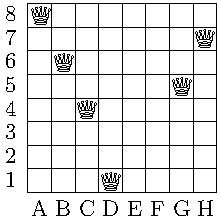
\includegraphics[scale=1]{examples/Chess2.pdf} \\
        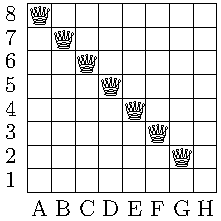
\includegraphics[scale=1]{examples/Chess3.pdf} &
        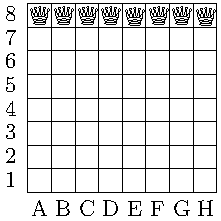
\includegraphics[scale=1]{examples/Chess4.pdf}
    \end{tabular}
\end{figure}

\begin{figure}[htb]
    \centering
    
\includegraphics[scale=0.25]{examples/400x400.png}
    \caption{This is an caption!}
\end{figure}



\section{Description}
    % !Mode:: "TeX:UTF-8"
\subsection{Description}
\begin{description}
    \item[API] Application Programming Interface
    \item[LAN] Local Area Network
    \item[ASCII] American Standard Code for Information Interchange
\end{description}

\section{Tables}
    % !Mode:: "TeX:UTF-8"
\subsection{Tables}
% http://tablesgenerator.com/
\begin{table}[ht]
    \centering
    \begin{tabular}{l | c | c | c | c }
    Competitor Name & Swim & Cycle & Run & Total \\
    \hline \hline
    John T & 13:04 & 24:15 & 18:34 & 55:53 \\
    Norman P & 8:00 & 22:45 & 23:02 & 53:47\\
    Alex K & 14:00 & 28:00 & n/a & n/a\\
    Sarah H & 9:22 & 21:10 & 24:03 & 54:35
    \end{tabular}
    \caption{Triathlon results}
\end{table}


\section{Definition}
    % !Mode:: "TeX:UTF-8"
% Package `amsthm'.
\subsection{Definition}
Then there’s the definition environment which produces a standard color block but with the title already specified as ‘definition’.
    \begin{verbatim}
    \begin{definition}
    A prime number is a number that...
    \end{definition}
    \end{verbatim}
\begin{defn}[Prime Number]
    A prime number is a number that...
\end{defn}


\section{Theorem}
    % !Mode:: "TeX:UTF-8" 
\subsection{Theorem Blocks}
\begin{thm}[Pythagoras]
    $ a^2 + b^2 = c^2$
\end{thm}
\begin{cor}
    $ x + y = y + x  $
\end{cor}
\begin{proof}
    $\omega +\phi = \epsilon $
\end{proof}



\section{Hyperlink}
    % !Mode:: "TeX:UTF-8"
\href{https://github.com/Iydon}{\faGithub}

\section{Bibliography}
    % !Mode:: "TeX:UTF-8"
\subsection{Bibliography}
\bibliographystyle{IEEEtran}
\nocite{*}

\bibliography{ref}


\section{Introduction}
    % !Mode:: "TeX:UTF-8" 
\lipsum[2]
\begin{itemize}
    \item minimizes the discomfort to the hands, or
    \item maximizes the outgoing velocity of the ball.
\end{itemize}
We focus exclusively on the second definition.
\begin{itemize}
    \item the initial velocity and rotation of the ball,
    \item the initial velocity and rotation of the bat,
    \item the relative position and orientation of the bat and ball, and
    \item the force over time that the hitter hands applies on the handle.
\end{itemize}
\lipsum[3]
\begin{itemize}
    \item the angular velocity of the bat,
    \item the velocity of the ball, and
    \item the position of impact along the bat.
\end{itemize}
\lipsum[4]
\emph{center of percussion} [Brody 1986], \lipsum[5]
\begin{Theorem}\label{thm:latex}
    \LaTeX
\end{Theorem}
\begin{Lemma} \label{thm:tex}
    \TeX .
\end{Lemma}
\begin{proof}
    The proof of theorem.
\end{proof}

\subsection{Other Assumptions}
\lipsum[6]
\begin{itemize}
    \item
    \item
    \item
    \item
\end{itemize}
\lipsum[7]
\section{Analysis of the Problem}
    % !Mode:: "TeX:UTF-8"
\begin{figure}[ht]
    \small
    \centering
    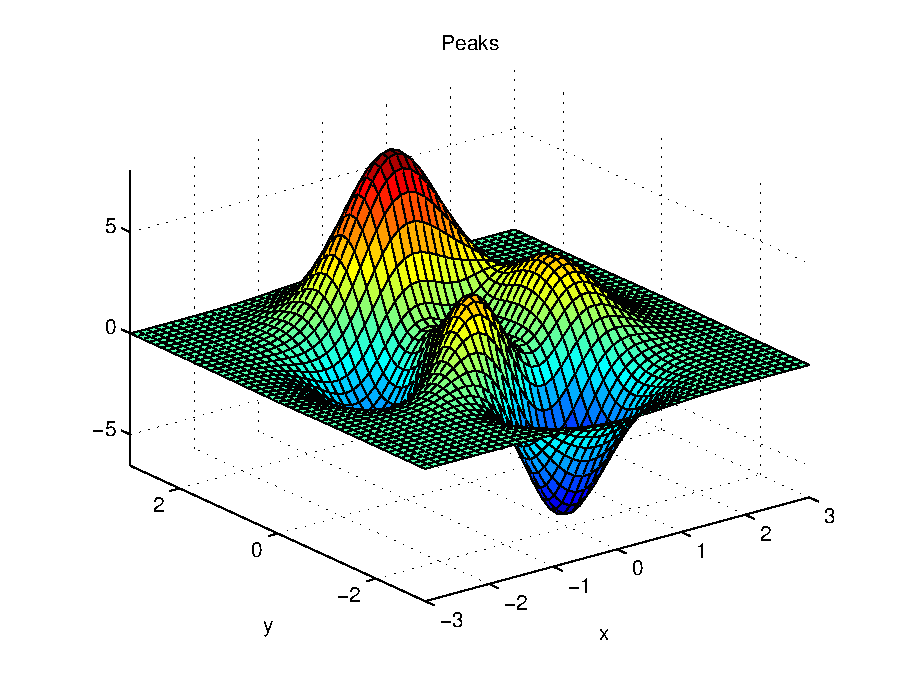
\includegraphics[width=12cm]{mcmthesis-aaa.eps}
    \caption{aa}\label{fig:aa}
\end{figure}
\lipsum[8] \eqref{aa}
\begin{equation}
    a^2 \label{aa}
\end{equation}
\[
    \begin{pmatrix}{*{20}c}
    {a_{11} } & {a_{12} } & {a_{13} }  \\
    {a_{21} } & {a_{22} } & {a_{23} }  \\
    {a_{31} } & {a_{32} } & {a_{33} }  \\
    \end{pmatrix}
    = \frac{{Opposite}}{{Hypotenuse}}\cos ^{ - 1} \theta \arcsin \theta
\]
\lipsum[9]
\[
    p_{j}=\begin{cases} 0,&\text{if $j$ is odd}\\
    r!\,(-1)^{j/2},&\text{if $j$ is even}
    \end{cases}
\]
\lipsum[10]
\[
    \arcsin \theta  =
    \mathop{{\int\!\!\!\!\!\int\!\!\!\!\!\int}\mkern-31.2mu
    \bigodot}\limits_\varphi
    {\mathop {\lim }\limits_{x \to \infty } \frac{{n!}}{{r!\left( {n - r}
    \right)!}}} \eqno (1)
\]

\section{Calculating and Simplifying the Model}
    % !Mode:: "TeX:UTF-8"
\lipsum[11]

\section{The Model Results}
    % !Mode:: "TeX:UTF-8"
\lipsum[6]

\section{Validating the Model}
    % !Mode:: "TeX:UTF-8"
\lipsum[9]

\section{Conclusions}
    % !Mode:: "TeX:UTF-8"
\lipsum[6]

\section{A Summary}
    % !Mode:: "TeX:UTF-8"
\lipsum[6]

\section{Evaluate of the Mode}
    % !Mode:: "TeX:UTF-8"
\lipsum[1]

\section{Strengths and weaknesses}
    % !Mode:: "TeX:UTF-8"
\lipsum[12]

\subsection{Strengths}
\begin{itemize}
\item \textbf{Applies widely}\\
This  system can be used for many types of airplanes, and it also
solves the interference during  the procedure of the boarding
airplane,as described above we can get to the  optimization
boarding time.We also know that all the service is automate.
\item \textbf{Improve the quality of the airport service}\\
Balancing the cost of the cost and the benefit, it will bring in
more convenient  for airport and passengers.It also saves many
human resources for the airline. \item \textbf{}
\end{itemize}

% !Mode:: "TeX:UTF-8"
\begin{thebibliography}{99}
\bibitem{1} D.~E. KNUTH   The \TeX{}book  the American
Mathematical Society and Addison-Wesley
Publishing Company , 1984-1986.
\bibitem{2}Lamport, Leslie,  \LaTeX{}: `` A Document Preparation System '',
Addison-Wesley Publishing Company, 1986.
\bibitem{3}\url{http://www.latexstudio.net/}
\bibitem{4}\url{http://www.chinatex.org/}
\end{thebibliography}

\begin{appendices}
    % !Mode:: "TeX:UTF-8"
\section{First appendix}
\lipsum[13]
Here are simulation programmes we used in our model as follow.\\
\textbf{\textcolor[rgb]{0.98,0.00,0.00}{Input matlab source:}}
\lstinputlisting[language=Matlab]{./code/mcmthesis-matlab.m}

\section{Second appendix}
some more text \textcolor[rgb]{0.98,0.00,0.00}{\textbf{Input C++ source:}}
\lstinputlisting[language=C++]{./code/mcmthesis-sudoku.cpp}

\section{Third appendix}
\lstinputlisting[language=Python]{./code/mcmthesis-python.py} 
\end{appendices}

\end{document}
